\section{Test Population}
\label{chap:test_population}

The composition and selection of a test group is an important part affecting the result of a study. Therefore, before presenting the results, the type of people who tested the application will be given. As described in Chapter \ref{chap:execution}, we wanted to choose participants that could provide valuable data. Figure \ref{fig:gender_stats} and Figure \ref{fig:age_stats}  displays the distribution of gender and age among the participants.

\begin{figure}[H]
    \begin{minipage}{.5\textwidth}
      \centering
      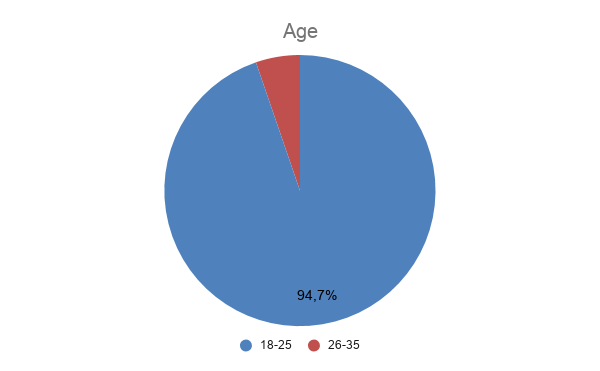
\includegraphics[width=\textwidth]{Images/Results/Population/Age.png}
      \captionof{figure}{Test group age distribution.}
      \label{fig:gender_stats}
    \end{minipage}
    \begin{minipage}{.5\textwidth}
      \centering
      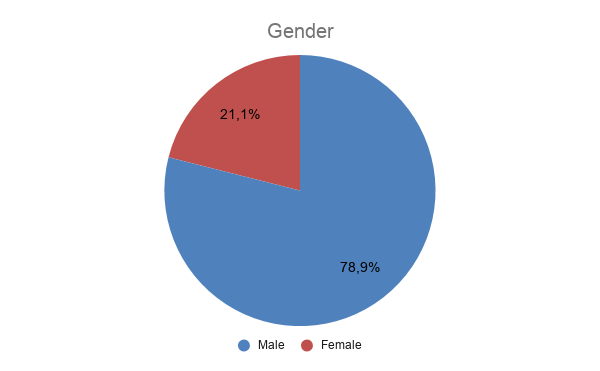
\includegraphics[width=\textwidth]{Images/Results/Population/Gender.png}
      \captionof{figure}{Test group gender distribution.}
      \label{fig:age_stats}
    \end{minipage}
    \vspace*{-\baselineskip}
\end{figure}

There were 19 participants in the study, 15 men and four women. All of them were students based in Trondheim, with a dominant age group of 18-25, and only one participant above this age.

\subsection{Sub-populations}
Since Hover is a concept highly dependent on the social aspect, we wanted to test it on people that knew each other before testing the application. We decided to choose two groups of people from our network in Trondheim, one based on student society volunteers, and another one consisting of classmates. The two groups gave us insights on how the social aspect affects the application usage, as described in \textit{RQ2}, \textit{RQ3}, and \textit{RQ4}.

\textbf{Student society volunteers}\\
The first group of  participants is volunteers  at the student society (samfundet) in Trondheim. The participants consist of 11 men and one woman. The group is tightly connected, working together a lot, including approximately three regular meetings every week. Thus, their social relationship is strong.

\textbf{Classmates}\\
The second group consists of seven people recruited from our study program at NTNU, four men and three women. Participants in this group know each other to various degrees. Some of them are very close and meet each other every day, while others probably did not speak together during the test period. Therefore, the relationship in the group is a lot weaker than in the student society group. Chapter \ref{chap:player_engagement}, Chapter \ref{chap:player_enjoyment}, and Chapter \ref{chap:player_motivation} will present the study with differences between the two groups which will be further discussed in Chapter \ref{chap:discussion}

\subsection{Interviews}
As a part of the testing, we also conducted single and group interviews to get more concrete feedback and statements from the participants. The subjects for these interviews were recruited from the population of people who had tested the application. In total, five people were interviewed.

\subsection{Summary}
In this chapter, an overview of which people the application was tested on has been described. The next chapters will introduce the result from the test period, presenting them according to the research questions.